\FloatBarrier
\section{Introduction}

\begin{figure}[t!]
\centering
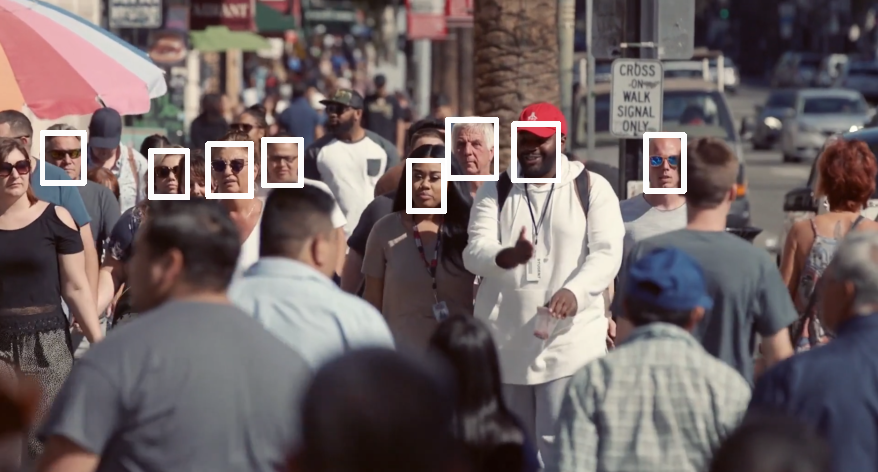
\includegraphics[width=\linewidth]{example_scene.pdf}
\caption{Example of crowded video-surveillance scenario targeted in this work. Faces (white bounding boxes) are most of the time the only visible part of the subjects to be tracked. In this scenario, the proposed face tracking approach surpasses general object tracking methods.}
\label{fig:crowded_onlyfaces}
\end{figure}

Recent advances on Convolutional Neural Networks (CNNs) and improvements on IP cameras (e.g. new lenses, 4K/8K resolutions) have allowed to move video-surveillance systems to increasingly crowded, large-scale and unconstrained scenarios.    
These novel scenarios typically involve crowds of people massively walking toward cameras located at near eye level, as illustrated in Figure~\ref{fig:crowded_onlyfaces}. 

When a face recognition system is deployed, alarms are sent to end-users (e.g. police bodies) every time a new subject is detected or identified. The subject is generally tracked, and one single alarm is generated per track to avoid sending multiple duplicate alarms. Obtaining long tracks is therefore of the utmost importance to increase the system's usability.  Moreover, a subject may remain on scene for seconds or even minutes. Making enforcement bodies wait until the end of tracks to receive alerts (which is known as \textit{offline} strategy) implies losing a precious time that could save lives. Hence, real-time and online constraints become essential. However, in this context, it is particularly challenging to perform reliable online long-term tracking of subjects, since: 

\begin{itemize}
    \item The face is often the only visible part of the person. Consequently, the tracking algorithm has to rely on the facial region exclusively, and not on more extended full-body or upper-body regions as in classic pedestrian tracking works \cite{li2014datasetCUHK,chen2019integrated}.
    \item People in video-surveilled places typically move all around the scene, positioning themselves closer or farther from the camera focus, and becoming occluded or blurred for long periods. Existing generic object trackers cannot handle these situations properly, as demonstrated in \cite{lin2019mobiface}.
    \item There is a lack of available datasets covering this kind of scenarios. Crowded video-surveillance videos are particularly difficult to collect and annotate.
\end{itemize}

In this work, we propose an architecture especially conceived for long-term face tracking in crowded video-surveillance contexts. More specifically, our main contributions can be summarized as follows:

\begin{itemize}
    \item Our architecture recovers from partial and full long-term occlusions thanks to a novel online tracklet reconnection module grounded on face verification techniques.
    \item We also propose a track correction module, which updates past track assignments with current information. This module has no extra computational cost, while considerably improving long-term tracking performance.
    \item We validate the system with regard to different state-of-the-art trackers, and present an ablation study quantifying the contribution of each proposed module. Four validation metrics designed to evaluate long-term tracking capabilities are introduced for that purpose.
    \item We publicly release to the community the video dataset used in our experiments, including ground truth track annotations.
\end{itemize}

